%%==================================================
%% chapter05.tex for SJTU Master Thesis
%% based on CASthesis
%% modified by wei.jianwen@gmail.com
%% version: 0.3a
%% Encoding: UTF-8
%% last update: Dec 5th, 2010
%%==================================================

%\bibliographystyle{sjtu2} %[此处用于每章都生产参考文献]
\raggedbottom
\chapter{实验与分析}
\label{chap:evaluation}
%向下 或 向上 取整的小优化

% 1,单位长度的误差方差比对,3种  diffGen,已调整/未调整)。 设置高度,画5个图
% 横坐标 第i个叶子,纵坐标 标准差  x 4(4个高度,4,7,10,13)  1,1  0.5   递增,因为层数越高 代价越小 噪音越大
% 横坐标  高度,纵坐标平均每个叶子的标准差1,2

% 应该是 每个error(i),有new - baseline  与  noise - baseline。然后  sum[error(i)]

% 2,内部节点。一样 也是5个图
%\part{title} 横坐标 第i个节点,纵坐标 标准差  x 4(4个高度,4,7,10,13)2,1
% 横坐标  高度,纵坐标平均每个节点的标准差2,2



% 3, 范围查询 。首先还是单点,内部节点的单点。比对 已调整/未调整 的差别,此时不比叶节点了
% 然后是范围查询情况,扯扯淡 因为没法设计啊  好像能设计诶 。 通过 c45肯定可以说明
% 横坐标  范围从2,3,4.。。。。。。,纵坐标,对应的标准差   5个图   3


% 4,找个推荐算法

\section{引言}

在前面的章节,我们已经介绍了面向分类应用的差分隐私算法在范围计数查询需求中存在的噪音线性叠加的问题,探讨了问题的频率矩阵加噪模型本质。接着详细介绍基础算法DiffGen与基于直方图发布方式的优化方案,DiffGen的匿名化过程决定其拥有一致性特性,这是二者之间的联系基础。然后说明DiffGen具有一维直方图特性,从树状组织结构和一致性约束出发,设计并实现优化算法DiffCon。在DiffCon中,设计了新的应答查询模式和全局敏感性定义,并调整噪音分布已达到在单位和范围查询情况均获得较好性能的目的。最后从理论角度,由误差方差对优化性能做了讨论总结。

本章节将在多个方面对DiffCon算法做比对实验,通过真实数据集测试算法准确度性能,以及基于$TMSC$算查询应答模式的噪音误差方差表现。主要工作包括:实验数据集、平台介绍;实验方案的设计;就实验结果进行分析说明。

\section{实验平台及设置}

\subsection{实验平台介绍}

首先介绍实验的硬件环境:
\begin{enumerate}
	\item 处理器:Intel® Core™ i5-3470 @ 3.20GHz,拥有2个物理内核(Physical Core),利用Hyper-Threading技术实现4个逻辑内核(Logical Core)。
	\item 内存:16G
	\item 硬盘:500G
\end{enumerate}

软件环境为:
\begin{enumerate}
	\item 操作系统为Windows 7旗舰版
	\item 编码语言为C++,采用Microsoft Visual Studio Community 2013集成开发环境。
	\item 使用matplotlib绘图
\end{enumerate}

\subsection{数据集简介}

实验部分的所有测试均基于真实数据集Adult\footnote{\url{https://archive.ics.uci.edu/ml/datasets/Adult}}\cite{adult}。它共有48863个样本,由6个连续属性、8个离散属性构成,类属性是对收入水平的判断,有2个两属性值“$\leqslant$50$K$”和“$>$50$K$”。所有的属性及属性值显示如图\ref{fig:adult}:

\begin{figure}[!htp]
	\centering
	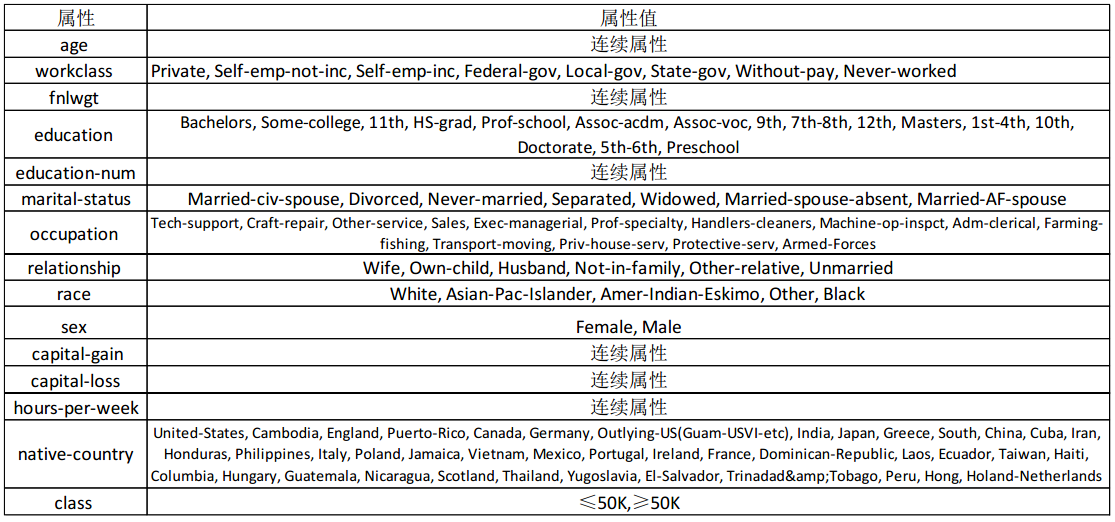
\includegraphics[width=5.8in]{chap5/adult}
	\bicaption[fig:adult]{图}{Adult数据集中的属性及属性值}{Fig.}{The attributes and attribte values in Adult dataset}
\end{figure}

由于在Adult数据集中存在着属性缺失的样本,因此在使用前需要进行处理。剔除不完整的样本之后,最终得到45222个可用的完整样本。

\section{实验设计概览}

本课题的目的是提升发布数据可用性,即提高数据在后续应用中的分类准确度,以此作为算法好坏的标准。因此,我们从理论测试和实践两个角度设计实验,概括如下:
\begin{enumerate}
	\item 验证理论分析结果。在\ref{theory analysis}节中,我们使用噪音的误差方差来评价算法的好与坏,作为衡量发布数据可用性的标杆。因此,在实验的第一部分中,我们比对三种不同应答查询模式下的误差方差:(1)往每个树节点加噪的初步方案$\tilde{L}_{all}(D)$。(2)基础算法DiffGen方式,即直方图模型$\mathcal{H}$,全局敏感性为1。(3)本课题的优化算法DiffCon方式$\tilde{\mathcal{H}}_{opt}$。在实验场景设计上,我们从单位长度查询和范围查询两个方面进行测试。方差能够使得两种数据的差距更加明显,但是,关注单一数据时,数据趋势的抖动会加剧,并且会导致实验图坐标的粒度太大,成倍淡化数值较小的数据分布特征。因此,采用标准差作为观察值。
	\item 真实分类算法上的实践。误差方差的理论测试难以替代真实场景的应用,因此通过C4.5分类器\cite{C45}来检测发布数据的分类准确度。同时,比对两个不同决策树分类算法的影响:IG(信息增益算法,Information Gain)和Max\cite{max}(最大值算法),最后分析实验结果。
\end{enumerate}	

\section{单位长度查询的测试与分析} 
\subsection{实验方案}
%跑几次,如何取平均
单位长度查询实验是基于同一$DTree$树结构,比对3种应答查询模式下叶节点计数值的误差方差。由于$DTree$可由树高控制,因此设定4种树高{4,7,10,13}场景。在每一种树高生成的$DTree$树中,分别抽取20,50,100,200个叶节点,统计每个叶节点上的误差标准差。
记节点$x$的的真实计数值为$C(x)$,初步方案下含噪计数值为$\tilde{L}_{all}(x)$,DiffGen方式下为$DiffGen(x)$,DiffCon方式下为$DiffCon(x)$。
实验算法如下:
\begin{algorithm}[H]
	\caption{单位长度查询实验}
	\begin{algorithmic}[1]
		\REQUIRE $DTree$树
		\ENSURE 叶节点数据项在三种查询应答模式下的误差标准差集合$\Upsilon_{all}$,$\Upsilon_{DiffGen}$,$\Upsilon_{DiffCon}$
		初始化, $\Upsilon_{all}$,$\Upsilon_{DiffGen}$,$\Upsilon_{DiffCon}$ $\leftarrow$ $\varnothing$
		\FOR{$DTree$中的第i个叶节点$leaf_{i}$}
		\STATE $\Upsilon_{all}$ $\leftarrow$ $\Upsilon_{all}$ $\bigcup$ $\sqrt {(\tilde{L}_{all}(leaf_{i})-C(leaf_{i}))^2}$
		\STATE $\Upsilon_{DiffGen}$ $\leftarrow$ $\Upsilon_{DiffGen}$ $\bigcup$ $\sqrt {(DiffGen(leaf_{i})-C(leaf_{i}))^2}$
		\STATE $\Upsilon_{DiffCon}$ $\leftarrow$ $\Upsilon_{DiffCon}$ $\bigcup$ $\sqrt {(DiffCon(leaf_{i})-C(leaf_{i}))^2}$
		\ENDFOR
		\RETURN $\Upsilon_{all}$,$\Upsilon_{DiffGen}$,$\Upsilon_{DiffCon}$
	\end{algorithmic}
\end{algorithm}



%平均单位长度的设计

\subsection{实验结果及分析}

单位长度查询的实验结果如图\ref{fig:EachLeaf},对树高Tree Height = 4,7,10,13的情况分别进行了测试,三种查询应答模式与图例中的标记对应关系如表\ref{chap5_table1}。横坐标是枚举每个抽取到的叶节点,坐标值x表示$Dtree$的第x个叶节点,也就是第x个单位长度数据项;纵坐标是误差标准差的计算值,坐标值y越大,表示标准差越大,单位查询结果稳定性越差,也就是偏离真实结果的距离越大,准确度越低。

\begin{table}[!hpb]
	\label{chap5_table1}
	\centering
		\bicaption[tab:firstone]{表}{查询应答模式与图例标记的对应关系表}{Table}{The relational table between inquiry-response mode and legend}
		\begin{tabular}{|c|c|c|}
			\hline
			$\textbf{查询应答模式}$ & $\textbf{图例标记}$\\
			\hline
			$\tilde{L}_{all}(D)$ & $\tilde{L}_{all}$ \\
			\hline
			DiffGen($\mathcal{H}$) & DiffGen \\
			\hline
			DiffCon($\tilde{\mathcal{H}}_{opt}$) & DiffCon \\
			\hline
		\end{tabular}
\end{table}


\begin{figure}[!htp]
	\centering
	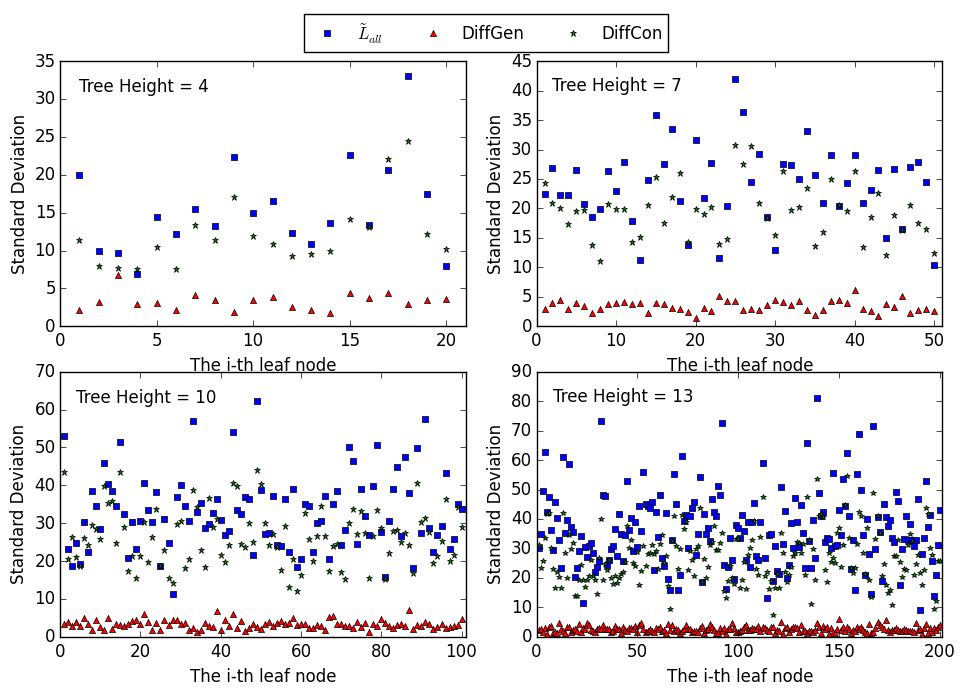
\includegraphics[width=5.5in]{chap5/EachLeaf}
	\bicaption[fig:EachLeaf]{图}{单位长度查询的实验结果}{Fig.}{The experimental result for unit-length queries}
\end{figure}

从实验结果来看,可观测到3个实验现象:(1)对于单位长度查询需求而言,DiffGen返回的应答结果距离真实值最近,并且分布相对稳定。(2)$\tilde{L}_{all}$和DiffCon都不是很稳定,在应答结果准确度上DiffCon优于DiffGen---对于同一X值,绝大部分的DiffCon点的Y值小于DiffGen的,树高4和7的实验结果比较容易看出。(3)随着树高的增加,误差标准差递增(在下个实验中更容易看出)。

导致DiffCon和$\tilde{L}_{all}$的误差标准差分布不稳定以及在应答准确度上均劣于DiffGen的原因,主要在于全局敏感性较大的缘故,都是树高$TH$。更大的全局敏感性决定了需要添加更多的噪音,在每个节点上$Laplace(TH/\varepsilon)$的量级,显然大于DiffGen的$Laplace(1/\varepsilon)$,因此更多的噪音扰动自然而然降低了应答准确度。同时,由于拉普拉斯概率密度函数是按照指数分布变动的布朗运动,更大的全局敏感性导致的是指数式的概率增减,必然加剧了函数结果的随机性,所以$\tilde{L}_{all}$和DiffCon不稳定。

\begin{figure}[!htp]
	\centering
	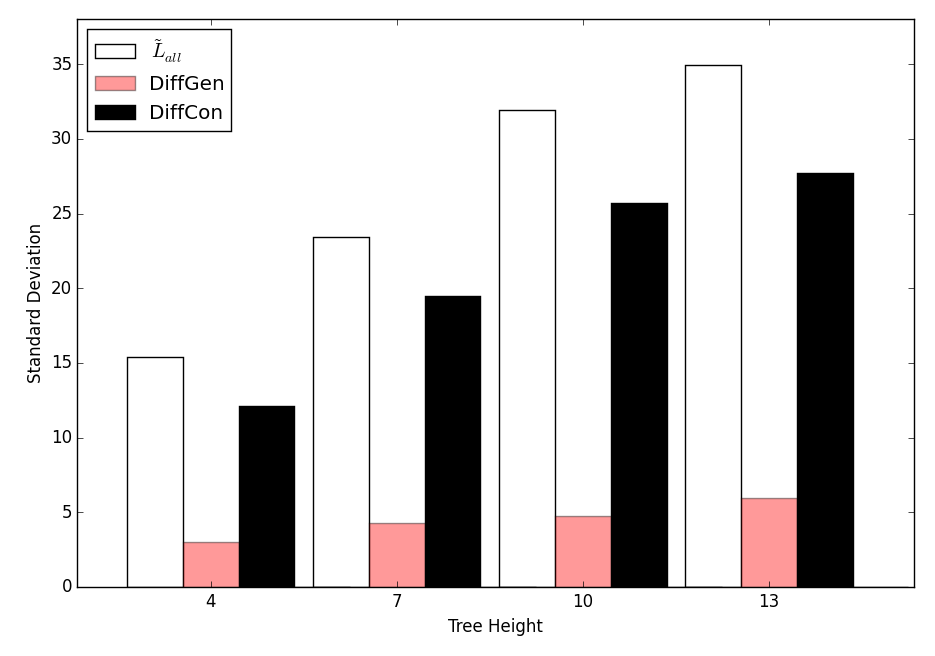
\includegraphics[width=5.3in]{chap5/average_eachleaf}
	\bicaption[fig:average_eachleaf]{图}{单位长度查询的实验结果}{Fig.}{The experimental result for unit-length queries}
\end{figure}

平均单位长度查询的误差标准差实验结果如图\ref{fig:average_eachleaf},横坐标表示树高,纵坐标表示误差标准差的计算值。由实验结果观察到2个现象:(1)DiffGen返回的应答结果准确度最优,DiffCon次之,$\tilde{L}_{all}$最差。此现象的原因分析前文已论述过。(2)三种应答查询模式随着树高的增加,误差标准差随之增加(DiffGen起伏较小,但经多组实验观测也满足这个规律),产生这个现象的原因在于全局敏感性的定义上。随着树高的增加,由于$DTree$构建算法\ref{diffgen}中需要对隐私代价$\varepsilon$根据树高进行切分。显然,随着树高的增加,切分得越细,作为加噪参数分母部分的${\varepsilon}'$越小,噪音量级$Laplace(S(\mathcal{F})/{\varepsilon}')$越大。



\section{范围查询的测试与分析}
\subsection{实验方案}

\begin{algorithm}[H]
	\caption{范围查询实验}
	\begin{algorithmic}[1]
		\REQUIRE $DTree$树
		\ENSURE 叶节点数据项在三种查询应答模式下的误差标准差集合$\Upsilon_{all}$,$\Upsilon_{DiffGen}$,$\Upsilon_{DiffCon}$
		初始化, $\Upsilon_{all}$,$\Upsilon_{DiffGen}$,$\Upsilon_{DiffCon}$ $\leftarrow$ $\varnothing$
		\FOR{$DTree$中的第i个叶节点$leaf_{i}$}
		\STATE $\Upsilon_{all}$ $\leftarrow$ $\Upsilon_{all}$ $\bigcup$ $\sqrt {(\tilde{L}_{all}(leaf_{i})-C(leaf_{i}))^2}$
		\STATE $\Upsilon_{DiffGen}$ $\leftarrow$ $\Upsilon_{DiffGen}$ $\bigcup$ $\sqrt {(DiffGen(leaf_{i})-C(leaf_{i}))^2}$
		\STATE $\Upsilon_{DiffCon}$ $\leftarrow$ $\Upsilon_{DiffCon}$ $\bigcup$ $\sqrt {(DiffCon(leaf_{i})-C(leaf_{i}))^2}$
		\ENDFOR
		\RETURN $\Upsilon_{all}$,$\Upsilon_{DiffGen}$,$\Upsilon_{DiffCon}$
	\end{algorithmic}
\end{algorithm}


\subsection{实验结果及分析}

\section{面向分类算法的测试与分析}

\subsection{实验方案}

\subsection{实验结果及分析}    

\section{本章小结}

